\documentclass{article}
\usepackage{amsmath}
\usepackage[margin=1in]{geometry}
\setlength\parindent{0pt}
\usepackage{amssymb,amscd,graphicx}
\usepackage{hyperref}
\usepackage{float}
\usepackage{mathrsfs}  
\usepackage{color}
\usepackage[]{amsmath}
\usepackage{amsfonts}
\usepackage{amsthm}
\bibliographystyle{unsrt}
\usepackage{amssymb}
\title{Math 371 Final Exam (take home part) }
\date
\Large
\begin{document}
	\maketitle
	\large
	\section{Guide: read carefully before you start}
	\begin{enumerate}
		\item Content: for each numerical method listed, write down a full summary as shown in the template.
		\item Format: this exam must be typed in LaTeX, which can be downloaded at \url{https://www.latex-project.org/}. This guideline will also serve as a template for LaTeX.
		\item You are required to keep this document up to date. It will be collected before the final exam. 
		\item Many quiz and the exam questions will come from this document.
		\item It's recommended that you keep a record of this document for the rest of your life.
		\item This part worths 50 points and requires an individual submission via google drive.
	\end{enumerate}
	\section{Numerical method list}
	\begin{itemize}
		\item done
		\item Bisection method \checkmark
		\item Newton's method \checkmark
		\item Secant method \checkmark
		\item Linear interpolation \checkmark
		\item Vandermonde matrix method \checkmark
		\item Newton interpolating polynomial \checkmark
		\item Lagrange interpolating polynomial \checkmark
		\item Linear spline function \checkmark
		\item Natural cubic spline function \checkmark
		\item Numerical approximation of the first derivative \checkmark
		\item Numerical integration using left point formula and midpoint formula
		\item Trapezoid rule \checkmark
		\item Simpson's rule \checkmark
		\item Adaptive Simpson's rule \checkmark
		\item Gaussian quadrature formula \checkmark
		\item Naive Gaussian elimination \checkmark
		\item Gaussian elimination with partial and full pivoting \checkmark
		\item LU factorization \checkmark
		\item Forward and backward Euler's method to solve differential equation \checkmark

	\end{itemize}
	\section{Summaries}
	\subsection{Bisection method:}
	This is a template. Your other summaries should follow the same format and answer all the questions (bold font) as listed in this template if applicable. Most of the content can be find in the lecture slides. Use your own resource to fill in the missing parts.\\
	
	{\bf Area of application:} bisection method is used to find the roots of a given equation.\\
	
	{\bf Mathematical theorem:} The Intermediate Value Theorem: \\[0.1in]
	If $f(x)$ is continuous on $[a,b]$ with $f(a)\cdot f(b)<0$, then $f(x) = 0$ for some $x$ in $[a,b]$.\\
	
	{\bf Idea of the method:} 
	\begin{enumerate}
		\item Find an interval $[a,b]$ with $f(a)\cdot f(b)<0$.
		\item Let $c$ be the middle point of $[a,b]$.
		\item Compute $f(c)$,
		\begin{itemize}
			\item If $f(c)\cdot f(a) <0$ choose the next interval to be $[a,c]$.
			\item If $f(c)\cdot f(b) <0$ choose the next interval to be $[c,b]$.
		\end{itemize}
		\item Repeat this procedure until it converges.
	\end{enumerate}
	{\bf Pseudocode:} (you can merge this part with the Matlab code. In the quiz, I will always ask for pseudocode since it's easier compared to Matlab code.)
	\begin{verbatim}
	function bisection(f,a,b,tol)
	
	a = a0, b = b0, tol = 1e-05;
	while (|a-b| > tol)
	c = (a+b)/2;
	if f(c) * f(a) < 0
	b = c;
	else
	a = c;
	end
	x = c;
	return x;
	\end{verbatim}
	{\bf Matlab code:} (compared to pseudocode, your code here should be written in the right grammar of Matlab and guaranteed to run. You also need to consider various invalid cases and display error messages.)
	\begin{verbatim}
	function x = bisection(f,a,b,tol)
	
	if (f(a)*(b)>=0)
	display('f(a) and f(b) have the same sign. Please use different a,b')
	return
	end
	while(abs(a-b)>tol)
	c = 1/2*(a+b);
	if (f(c) ==0);
	break;
	elseif (f(c)*f(a)<0)
	b = c;
	else
	a = c;
	end
	end
	
	x = c;
	\end{verbatim}
	{\bf Numerical analysis}
	\begin{itemize}
		\item{\bf When does it converge:} the method will always converge as long as
		\begin{itemize}
			\item $f(x)$ is continuous on $[a,b]$.
			\item $f(a)\cdot f(b)<0$.
		\end{itemize}
		\item {\bf Error estimate:} (write down the detailed derivation of the error estimate formula)
		\begin{equation}
		\begin{split}
		& E_0  < b-a,\quad
		E_{k+1}  < \frac{1}{2}E_k,\\
		\Rightarrow&\quad E_n <\frac{b-a}{2^n}.
		\end{split}
		\end{equation}
		\item {\bf Pros \& Cons:} (you are encouraged to search online for more inputs)
		\begin{itemize}
			\item Easy to use.
			\item Always converge.
			\item In the situation of multiple roots available, a carefully chosen starting interval $[a,b]$ is required to find a particular root.
			\item Slow.
			\item Only works for one dimension.
		\end{itemize}
	\end{itemize}
	{\bf Numerical experiment:}
	Test bisection method with 
	$$
	f(x) = x^3+2x-3,\quad a = -3, \quad b= 2,\quad r = 1.
	$$
	We obtain the error table\\[0.1in]
	\begin{tabular}{|c|c|c|c|c|c|c|c|}
		\hline
		Number of iterations & 1 & 2 & 3 & 4 & 5 & 6 & 7\\
		\hline
		Relative Error & 1.500000  & 0.250000  & 0.375000 & 
		0.062500  & 0.093750 & 0.015625 & 0.023438\\
		\hline
	\end{tabular}
	\\[0.1in]
	The convergence rate graph is (your graph should contain
	a title, x-label and y-label.)
	\begin{figure}[H]
		\caption{Convergence rate of bisection method}
		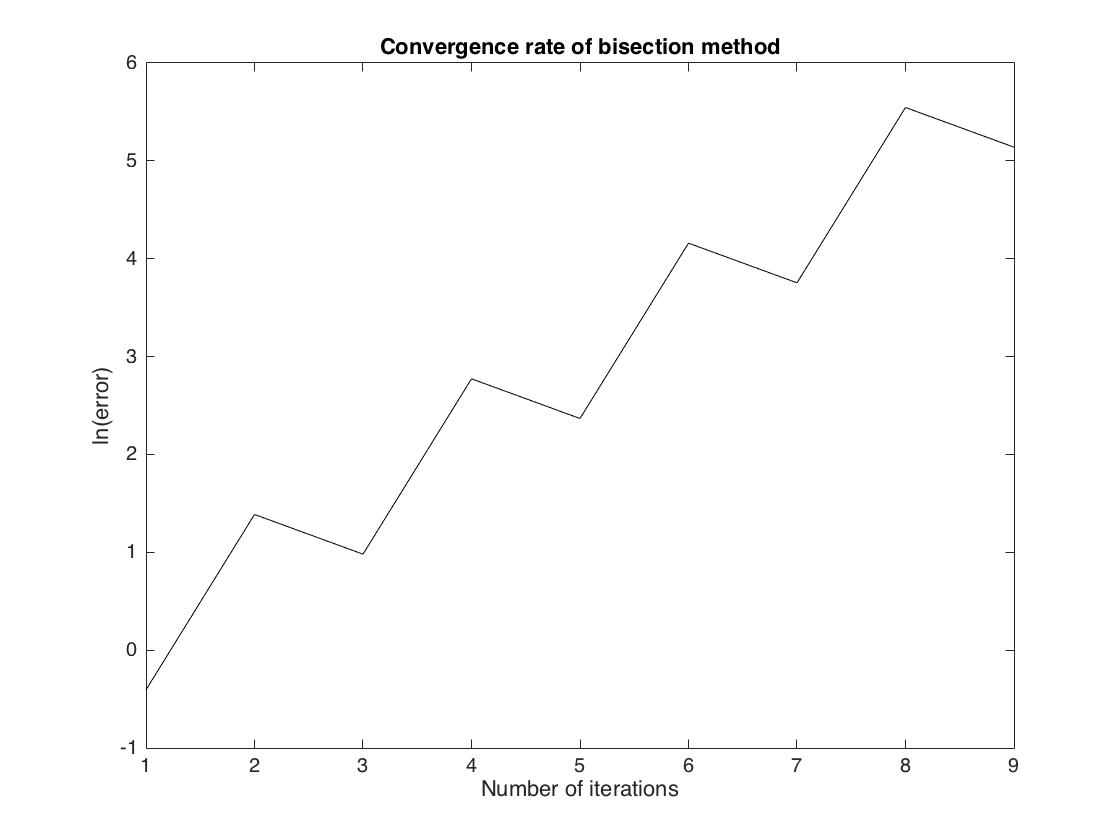
\includegraphics[width=0.8\textwidth, height=0.6\textwidth]{bisection_errorplot.jpg}
	\end{figure}
	\subsection{Newton Method:}
	
	{\bf Area of application:} Newton method is used to find the roots of a given equation.\\
	
	{\bf Mathematical theorem:} The Intermediate Value Theorem: \\[0.1in]
	If $f(x)$ is continuous on $[a,b]$ with $f(a)\cdot f(b)<0$, then $f(x) = 0$ for some $x$ in $[a,b]$.\\
	
	{\bf Idea of the method:} 
	The idea is to start with an initial guess which is reasonably close to the true root, then to approximate the function by its tangent line using calculus, and finally to compute the x-intercept of this tangent line by elementary algebra.\\
	\[x _ { n + 1 } = x _ { n } - \frac { f \left( x _ { n } \right) } { f ^ { \prime } \left( x _ { n } \right) }\]
	{\bf Code:}
	\begin{verbatim}
	function retval = newton (f,upper,tol)
	x = upper;
	while (abs(f(x)) > tol)
	x=x-(f(x)/deriv(f,x))
	endwhile
	retval = x;
	endfunction
	\end{verbatim}
	{\bf Numerical analysis}
	\begin{itemize}
		\item{\bf When does it converge:} When the function is continuous and does not have the following
		\begin{itemize}
			\item Iteration point is stationary
			\item Starting point enters a cycle
			\item Derivative does not exist at root
			\item Discontinuous derivative
		\end{itemize}
		\item {\bf Error estimate:}
		\begin{equation}
		\begin{split}
		& |e_{n+1}\leq \frac{1}{2}\frac{max(|f''(x)|)}{min(|f'(x)|)}(e_n^2)=ce_n^2
		\end{split}
		\end{equation}
		\item {\bf Pros \& Cons:}
		\begin{itemize}
			\item Fast
			\item Accurate
			\item Doesn't always converge
			\item Needs a derivative
		\end{itemize}
	\end{itemize}
	{\bf Numerical experiment:}
	Test Newton method with 
	\begin{align*} f _ { 1 } ( x ) & = \sin ( x ) - x - 1 \\ f _ { 2 } ( x ) & = x ( 1 - \cos ( x ) ) \\ f _ { 3 } ( x ) & = e ^ { x } - x ^ { 2 } + 3 x - 2 \end{align*}
	
	\begin{tabular}{|c|c|c|}
		\hline 
		Function &
		Number of Iterations &
		Approximate Root
		\\ 
		\hline
		
		$f_1(x)$ & 5 &  -1.934563 \\
		\hline 
		$f_2(x)$ & 11 & 0.010980 \\
		\hline
		$f_3(x)$ & 3 & 0.257530 \\
		\hline
		
	\end{tabular}\\
	\\[0.1in]
	The convergence rate graph is
	\begin{figure}[H]
		\caption{Convergence rate of newtons method}
		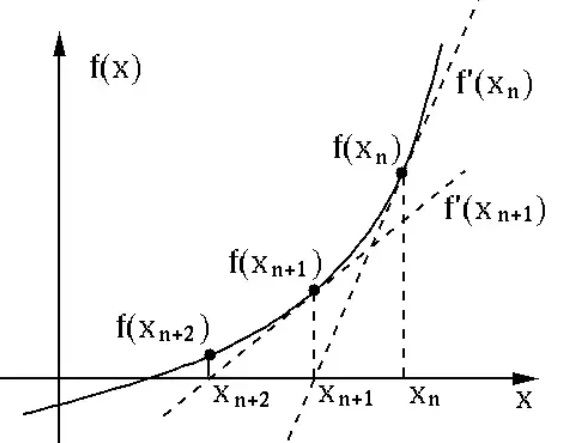
\includegraphics[width=0.8\textwidth, height=0.6\textwidth]{newtons_roots.jpg}
	\end{figure}
	\subsection{Secant Method:}
	
	{\bf Area of application:} Secant method is used to find the roots of a given equation.\\
	
	{\bf Mathematical theorem:} The Intermediate Value Theorem: \\[0.1in]
	If $f(x)$ is continuous on $[a,b]$ with $f(a)\cdot f(b)<0$, then $f(x) = 0$ for some $x$ in $[a,b]$.\\
	
	{\bf Idea of the method:} 
	In numerical analysis, the secant method is a root-finding algorithm that uses a succession of roots of secant lines to better approximate a root of a function f. 
	\[x _ { n } = x _ { n - 1 } - f \left( x _ { n - 1 } \right) \frac { x _ { n - 1 } - x _ { n - 2 } } { f \left( x _ { n - 1 } \right) - f \left( x _ { n - 2 } \right) } = \frac { x _ { n - 2 } f \left( x _ { n - 1 } \right) - x _ { n - 1 } f \left( x _ { n - 2 } \right) } { f \left( x _ { n - 1 } \right) - f \left( x _ { n - 2 } \right) }\]
	{\bf Code:}
	\begin{verbatim}
    function retval = secant (f,start1,start2,tol)
x = start1;
xPrev = start2;
while (abs(f(x)) > tol)
tmp = x;
x=x-f(x)*((x - xPrev)/(f(x)-f(xPrev)));
xPrev = tmp;
endwhile
retval = x;
endfunction
	\end{verbatim}
	{\bf Numerical analysis}
	\begin{itemize}
		\item{\bf When does it converge:} When the function is continuous and does not have the following
		\begin{itemize}
			\item Iteration point is stationary
			\item Starting point enters a cycle
			\item Derivative does not exist at root
			\item Discontinuous derivative
		\end{itemize}
		\item {\bf Error estimate:}
		\begin{equation}
		\begin{split}
		& |e_{n+1}\leq \frac{1}{2}\frac{f''(\xi_1)}{f'(\xi_2))}|e_n|\cdot |e_{n-1}) \leq c|e_n|\cdot|e_{n-1}|
		\end{split}
		\end{equation}
		\item {\bf Pros \& Cons:}
		\begin{itemize}
			\item Fast
			\item Accurate
			\item Doesn't always converge
			\item Needs a derivative
		\end{itemize}
	\end{itemize}
	{\bf Numerical experiment:}
	Test secant method with 
	\begin{align*} f _ { 1 } ( x ) & = \sin ( x ) - x - 1 \\ f _ { 2 } ( x ) & = x ( 1 - \cos ( x ) ) \\ f _ { 3 } ( x ) & = e ^ { x } - x ^ { 2 } + 3 x - 2 \end{align*}
	
\begin{tabular}{|c|c|c|}
	\hline 
	Function &
	Number of Iterations &
	Approximate Root
	\\ 
	\hline
	
	$f_1(x)$ & 6 &  -1.934563 \\
	\hline 
	$f_2(x)$ & 15 & 0.012283 \\
	\hline
	$f_3(x)$ & 3 & 0.257530 \\
	\hline
	
\end{tabular}\\
	\\[0.1in]
	The convergence rate graph is
	\begin{figure}[H]
		\caption{Convergence rate of secant method}
		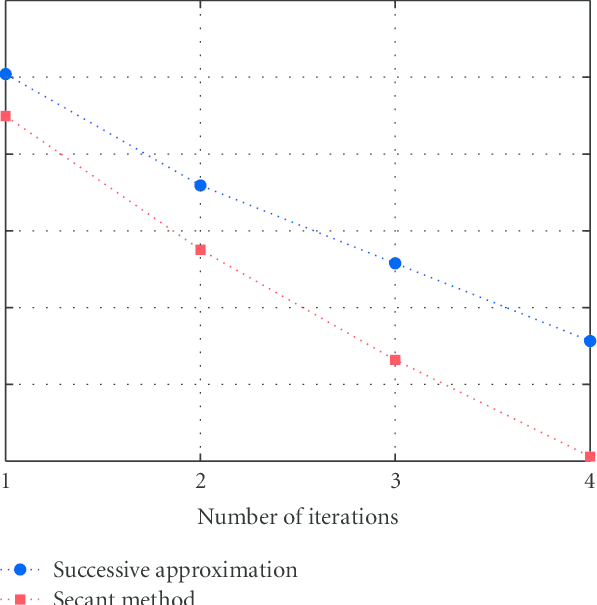
\includegraphics[width=0.8\textwidth, height=0.6\textwidth]{secant_method.png}
	\end{figure}

	\subsection{Linear Interpolation:}
	{\bf Area of application:}In mathematics, linear interpolation is a method of curve fitting using linear polynomials to construct new data points within the range of a discrete set of known data points.
	
	{\bf Idea of the method:} 
	If the two known points are given by the coordinates ${\displaystyle (x_{0},y_{0})} (x_{0},y_{0})$ and ${\displaystyle (x_{1},y_{1})} (x_{1},y_{1})$, the linear interpolant is the straight line between these points. For a value x in the interval ${\displaystyle (x_{0},x_{1})} (x_{0},x_{1}),$ the value y along the straight line is given from the equation of slopes.\\
	This formula can also be understood as a weighted average. The weights are inversely related to the distance from the end points to the unknown point; the closer point has more influence than the farther point. Thus, the weights are ${\textstyle {\frac {x-x_{0}}{x_{1}-x_{0}}}} {\textstyle {\frac  {x-x_{0}}{x_{1}-x_{0}}}}$ and ${\textstyle {\frac {x_{1}-x}{x_{1}-x_{0}}}} {\textstyle {\frac  {x_{1}-x}{x_{1}-x_{0}}}},$ which are normalized distances between the unknown point and each of the end points
	\[y = y _ { 0 } \left( 1 - \frac { x - x _ { 0 } } { x _ { 1 } - x _ { 0 } } \right) + y _ { 1 } \left( 1 - \frac { x _ { 1 } - x } { x _ { 1 } - x _ { 0 } } \right) = y _ { 0 } \left( 1 - \frac { x - x _ { 0 } } { x _ { 1 } - x _ { 0 } } \right) + y _ { 1 } \left( \frac { x - x _ { 0 } } { x _ { 1 } - x _ { 0 } } \right)\]
	{\bf Code:}
	\begin{verbatim}
function retval = linerInterpolation(f,a,b,tol)
while (abs(a-b) > tol)
slope = (f(b)-f(a))/(b-a)
line = @(x)slope*(x-a)+f(a);
guess = fzero(line,a);
if f(guess) * f(a) > 0
a = guess
else
b = guess
endif
endwhile
retval = guess;
endfunction
	\end{verbatim}
	{\bf Numerical analysis}
	\begin{itemize}
		\item{\bf When does it converge:} Provided we have the proper data, linear interpolation always converges.
		\item {\bf Error estimate:}
		\begin{equation}
		\begin{split}
		& |f (x) − P1(x)| \leq \frac{h^2}{8}
		max|f''(x)|, x \in [x0, x1].
		\end{split}
		\end{equation}
		\item {\bf Pros \& Cons:}
		\begin{itemize}
			\item Can fit most data
			\item Is not smooth unless taken a high number of times
		\end{itemize}
	\end{itemize}
	{\bf Numerical experiment:}
	Test interpolation method with 
	\begin{align*} f _ { 1 } ( x ) & = \sin ( x ) - x - 1 \\ f _ { 2 } ( x ) & = x ( 1 - \cos ( x ) ) \\ f _ { 3 } ( x ) & = e ^ { x } - x ^ { 2 } + 3 x - 2 \end{align*}
	
\begin{tabular}{|c|c|c|}
	\hline 
	Function &
	Number of Iterations &
	Approximate Root
	\\ 
	\hline
	
	$f_1(x)$ & 12 &  -1.934563 \\
	\hline 
	$f_2(x)$ & 500 & 0.051707 \\
	\hline
	$f_3(x)$ & 29 & 0.257530 \\
	\hline
	
\end{tabular}\\    
	\\[0.1in]
	The convergence rate graph is
	\begin{figure}[H]
		\caption{Convergence rate of liner interpolation}
		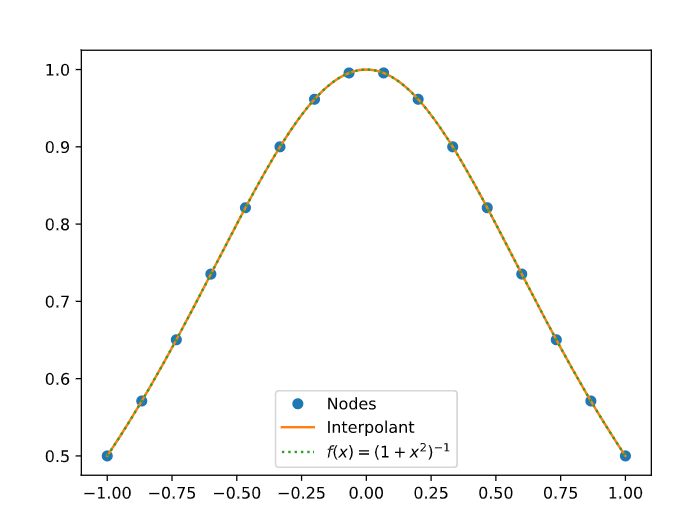
\includegraphics[width=0.8\textwidth, height=0.6\textwidth]{linear_interpolation.png}
	\end{figure}

	\subsection{Vandermonde Matrix:}
	{\bf Area of application:}In polynomial interpolation, since inverting the Vandermonde matrix allows expressing the coefficients of the polynomial in terms of the ${\displaystyle \alpha _{i}} $and the values of the polynomial at the$ {\displaystyle \alpha _{i}.}$
	
	{\bf Idea of the method:} 
	If the two known points are given by the coordinates ${\displaystyle (x_{0},y_{0})} (x_{0},y_{0})$ and ${\displaystyle (x_{1},y_{1})} (x_{1},y_{1})$, the linear interpolant is the straight line between these points. For a value x in the interval ${\displaystyle (x_{0},x_{1})} (x_{0},x_{1}),$ the value y along the straight line is given from the equation of slopes.\\
	This formula can also be understood as a weighted average. The weights are inversely related to the distance from the end points to the unknown point; the closer point has more influence than the farther point. Thus, the weights are ${\textstyle {\frac {x-x_{0}}{x_{1}-x_{0}}}} {\textstyle {\frac  {x-x_{0}}{x_{1}-x_{0}}}}$ and ${\textstyle {\frac {x_{1}-x}{x_{1}-x_{0}}}} {\textstyle {\frac  {x_{1}-x}{x_{1}-x_{0}}}},$ which are normalized distances between the unknown point and each of the end points
	\[y = y _ { 0 } \left( 1 - \frac { x - x _ { 0 } } { x _ { 1 } - x _ { 0 } } \right) + y _ { 1 } \left( 1 - \frac { x _ { 1 } - x } { x _ { 1 } - x _ { 0 } } \right) = y _ { 0 } \left( 1 - \frac { x - x _ { 0 } } { x _ { 1 } - x _ { 0 } } \right) + y _ { 1 } \left( \frac { x - x _ { 0 } } { x _ { 1 } - x _ { 0 } } \right)\]
	{\bf Code:}
	\begin{verbatim}
function A = VanInverse(B)
% This function inverse a Vandermonde Matrix B. 
% Matrix B is a n-by-n matrix, its (i,j) entry is i^(j-1),
% where i,j = 1,2,...,n
% for example, n = 4
% B =
%     1     1     1     1
%     1     2     4     8
%     1     3     9    27
%     1     4    16    64
% This routine uses a Stirling polynomial(the first kind) coefficients
% For fast operation, a C Stirling coefficient function has
% been posted with name: mStirling.c. The C-version of this 
% inverse function is also available upon request.
n = size(B,1);
A = zeros(n,n);
% compute the Stirling coeffs (by column), could use mStirling.c
for (i=1:n)
if (i==1) 
k = 3;
coeff = [1 -2];
else
k = 2;
coeff = [1 -1];
end
while (k<=n)
if (k == i);
k = k + 1;
continue;
else
coeff = conv(coeff, [1 -k]);
k = k + 1;
end
end
A(:,i) = coeff' .* ((-1).^(n-i)/(factorial(n-i)*factorial(i-1)));
end
A = flipud(A);
	\end{verbatim}
	{\bf Numerical analysis}
	\begin{itemize}
		\item{\bf When does it converge:} Provided we have the proper data, linear interpolation always converges.
		\item {\bf Error estimate:}
		\begin{equation}
		\begin{split}
		& \pi(x) = (x − x_1)(x − x_2)\cdots(x − x_n)
		\end{split}
		\end{equation}
		\item {\bf Pros \& Cons:}
		\begin{itemize}
			\item Nice Structure
			\item Expensive
			\item Matrix is ill-conditioned
		\end{itemize}
	\end{itemize}
	{\bf Numerical experiment:}
	$3x^2 − 5x + 7$ at the points (1,5) and (3,19)
	
\begin{tabular}{|c|c|c|}
	\hline 
	Function &
	Number of Iterations &
	Approximate
	\\ 
	\hline
	
	$f_1(x)$ & 23 &  5.425501 \\
	\hline
	
\end{tabular}\\    
	\\[0.1in]
	The convergence rate graph is
	\begin{figure}[H]
		\caption{Convergence rate}
		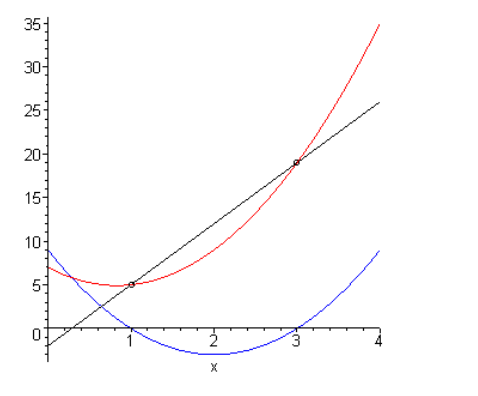
\includegraphics[width=0.8\textwidth, height=0.6\textwidth]{vandermonder.png}
	\end{figure}
	\subsection{Newton Interpolating Polynomial:}
	{\bf Area of application:}An interpolation polynomial for a given set of data points. The Newton polynomial is sometimes called Newton's divided differences interpolation polynomial because the coefficients of the polynomial are calculated using Newton's divided differences method.
	
	{\bf Idea of the method:} 
Solving an interpolation problem leads to a problem in linear algebra where we have to solve a system of linear equations. Using a standard monomial basis for our interpolation polynomial we get the very complicated Vandermonde matrix. By choosing another basis, the Newton basis, we get a system of linear equations with a much simpler lower triangular matrix which can be solved faster.
	{\bf Code:}
	\begin{verbatim}
function fp = newton_interpolation(x,y,p)
% Script for Newton's Interpolation.
% Muhammad Rafiullah Arain
% Mathematics & Basic Sciences Department
% NED University of Engineering & Technology - Karachi
% Pakistan.
% ---------
% x and y are two Row Matrices and p is point of interpolation
%
% Example
% >> x=[1,2,4,7,8]
% >> y=[-9,-41,-189,9,523]
% >> newton_interpolation(x, y, 5)
% OR
% >> a = newton_interpolation(x, y, 5)
n = length(x);
a(1) = y(1);
for k = 1 : n - 1
d(k, 1) = (y(k+1) - y(k))/(x(k+1) - x(k));
end
for j = 2 : n - 1
for k = 1 : n - j
d(k, j) = (d(k+1, j - 1) - d(k, j - 1))/(x(k+j) - x(k));
end
end
d
for j = 2 : n
a(j) = d(1, j-1);
end
Df(1) = 1;
c(1) = a(1);
for j = 2 : n
Df(j)=(p - x(j-1)) .* Df(j-1);
c(j) = a(j) .* Df(j);
end
fp=sum(c);

	\end{verbatim}
	{\bf Numerical analysis}
	\begin{itemize}
		\item{\bf When does it converge:} Provided we have the proper data; always converges.
		\item {\bf Error estimate:}
		\begin{equation}
		\begin{split}
		& p _ { n } ( z ) = \left( \begin{array} { l } { z } \\ { n } \end{array} \right) = \frac { z ( z - 1 ) \cdots ( z - n + 1 ) } { n ! }
		\end{split}
		\end{equation}
		\item {\bf Pros \& Cons:}
		\begin{itemize}
			\item Intuitive
			\item fast
			\item accurate
			\item must be differentiable
		\end{itemize}
	\end{itemize}
	{\bf Numerical experiment:}
		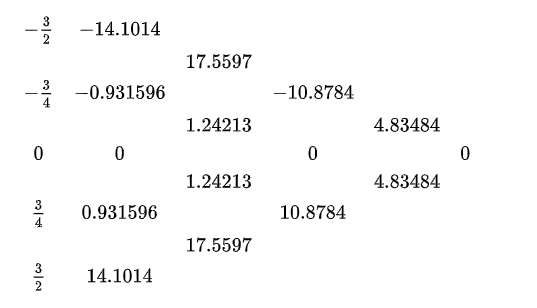
\includegraphics[width=0.8\textwidth, height=0.6\textwidth]{newton_poly_ex.png}
	$- 14.1014 + 17.5597 \left( x + \frac { 3 } { 2 } \right) - 10.8784 \left( x + \frac { 3 } { 2 } \right) \left( x + \frac { 3 } { 4 } \right) + 4.83484 \left( x + \frac { 3 } { 2 } \right) \left( x + \frac { 3 } { 4 } \right) ( x ) + 0 \left( x + \frac { 3 } { 2 } \right) \left( x + \frac { 3 } { 4 } \right) ( x ) \left( x - \frac { 3 } { 4 } \right) =$
	$\quad = - 0.00005 - 1.4775 x - 0.00001 x ^ { 2 } + 4.83484 x ^ { 3 }$

	The convergence rate graph is
	\begin{figure}[H]
		\caption{Convergence rate}
		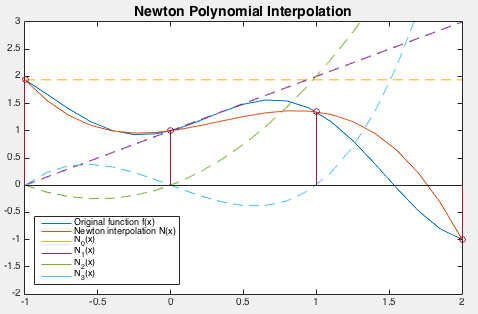
\includegraphics[width=0.8\textwidth, height=0.6\textwidth]{NewtonInterpolationEx.png}
	\end{figure}
	\subsection{Lagrange interpolating polynomial:}
{\bf Area of application:}In numerical analysis, Lagrange polynomials are used for polynomial interpolation. For a given set of points $ {\displaystyle (x_{j},y_{j})} {\displaystyle (x_{j},y_{j})}  $with no two $ {\displaystyle x_{j}} x_{j}  $values equal, the Lagrange polynomial is the polynomial of lowest degree that assumes at each value$  {\displaystyle x_{j}} x_{j} $ the corresponding value$  {\displaystyle y_{j}} y_{j} $ (i.e. the functions coincide at each point). The interpolating polynomial of the least degree is unique, 

{\bf Idea of the method:} 
Given a set of k + 1 data points

$ 	{\displaystyle (x_{0},y_{0}),\ldots ,(x_{j},y_{j}),\ldots ,(x_{k},y_{k})} (x_{0},y_{0}),\ldots ,(x_{j},y_{j}),\ldots ,(x_{k},y_{k}) $
where no two $ {\displaystyle x_{j}} x_{j} $ are the same, the interpolation polynomial in the Lagrange form is a linear combination. Thus,
\[\ell _ { j } ( x ) : = \prod _ { 0 \leq m \leq k \atop m \neq j } \frac { x - x _ { m } } { x _ { j } - x _ { m } } = \frac { \left( x - x _ { 0 } \right) } { \left( x _ { j } - x _ { 0 } \right) } \cdots \frac { \left( x - x _ { j - 1 } \right) } { \left( x _ { j } - x _ { j - 1 } \right) } \frac { \left( x - x _ { j + 1 } \right) } { \left( x _ { j } - x _ { j + 1 } \right) } \cdots \frac { \left( x - x _ { k } \right) } { \left( x _ { j } - x _ { k } \right) }\]
{\bf Code:}
\begin{verbatim}
function y=lagrange(x,pointx,pointy)
%
%LAGRANGE   approx a point-defined function using the Lagrange polynomial interpolation
%
%      LAGRANGE(X,POINTX,POINTY) approx the function definited by the points:
%      P1=(POINTX(1),POINTY(1)), P2=(POINTX(2),POINTY(2)), ..., PN(POINTX(N),POINTY(N))
%      and calculate it in each elements of X
%
%      If POINTX and POINTY have different number of elements the function will return the NaN value
%
%      function wrote by: Calzino
%      7-oct-2001
%
n=size(pointx,2);
L=ones(n,size(x,2));
if (size(pointx,2)~=size(pointy,2))
fprintf(1,'\nERROR!\nPOINTX and POINTY must have the same number of elements\n');
y=NaN;
else
for i=1:n
for j=1:n
if (i~=j)
L(i,:)=L(i,:).*(x-pointx(j))/(pointx(i)-pointx(j));
end
end
end
y=0;
for i=1:n
y=y+pointy(i)*L(i,:);
end
end
\end{verbatim}
{\bf Numerical analysis}
\begin{itemize}
	\item{\bf When does it converge:} Provided we have the proper data; always converges.
	\item {\bf Error estimate:}
	\begin{equation}
	\begin{split}
	&R ( x ) = \frac { \left( x - x _ { 0 } \right) \left( x - x _ { 1 } \right) \cdots \left( x - x _ { n } \right) f ^ { ( n + 1 ) } ( \xi ) } { ( n + 1 ) ! }
	\end{split}
	\end{equation}
	\item {\bf Pros \& Cons:}
	\begin{itemize}
		\item Intuitive
		\item Fast
		\item Accurate
	\end{itemize}
\end{itemize}
{\bf Numerical experiment:}
Approximating $ f(x)=x^2, 1\leq x\leq 3$
$\begin{array} { l l } { x _ { 0 } = 1 } & { f \left( x _ { 0 } \right) = 1 } \\ { x _ { 1 } = 2 } & { f \left( x _ { 1 } \right) = 4 } \\ { x _ { 2 } = 3 } & { f \left( x _ { 2 } \right) = 9 } \end{array}$
We get the polynomial
\[L ( x ) = 1 \cdot \frac { x - 2 } { 1 - 2 } \cdot \frac { x - 3 } { 1 - 3 } + 4 \cdot \frac { x - 1 } { 2 - 1 } \cdot \frac { x - 3 } { 2 - 3 } + 9 \cdot \frac { x - 1 } { 3 - 1 } \cdot \frac { x - 2 } { 3 - 2 }\]
The convergence rate graph is
\begin{figure}[H]
	\caption{Convergence rate}
	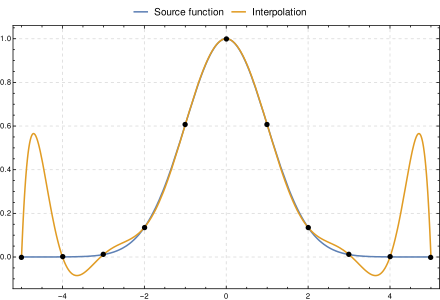
\includegraphics[width=0.8\textwidth, height=0.6\textwidth]{lagrange_poly.png}
\end{figure}
	\subsection{Linear spline function:}
{\bf Area of application:}Spline interpolation is a form of interpolation where the interpolant is a special type of piecewise polynomial called a spline. Spline interpolation is often preferred over polynomial interpolation because the interpolation error can be made small even when using low degree polynomials for the spline[1]. Spline interpolation avoids the problem of Runge's phenomenon, in which oscillation can occur between points when interpolating using high degree polynomials.

{\bf Idea of the method:} 
Taking a third-order polynomial $ q(x) $\\
$q ( x ) = ( 1 - t ( x ) ) y _ { 1 } + t ( x ) y _ { 2 } + t ( x ) ( 1 - t ( x ) ) ( a ( 1 - t ( x ) ) + b t ( x ) )$\\
Where\\
$t ( x ) = \frac { x - x _ { 1 } } { x _ { 2 } - x _ { 1 } }$
$a = k _ { 1 } \left( x _ { 2 } - x _ { 1 } \right) - \left( y _ { 2 } - y _ { 1 } \right)$
$b = - k _ { 2 } \left( x _ { 2 } - x _ { 1 } \right) + \left( y _ { 2 } - y _ { 1 } \right)$
We will take the derivatives and use those to build up linear equations. From that we will repeat as needed.\\
$q _ { n } ^ { \prime \prime } \left( x _ { n } \right) = - 2 \frac { 3 \left( y _ { n } - y _ { n - 1 } \right) - \left( 2 k _ { n } + k _ { n - 1 } \right) \left( x _ { n } - x _ { n - 1 } \right) } { \left( x _ { n } - x _ { n - 1 } \right) ^ { 2 } } = 0$
{\bf Code:}
\begin{verbatim}
    function s = LinearSpline (x, y)
s = zeros(length(x)-1, 4)
n = length(x);
for i = 1:n-1
m = (y(i+1)-y(i))./(x(i+1)-x(i));
b = -m*x(i)+y(i);
s(i,:) = [m b x(i) x(i+1)]
endfor
endfunction
\end{verbatim}
{\bf Numerical analysis}
\begin{itemize}
	\item{\bf When does it converge:} Provided we have the proper data; always converges.
	\item {\bf Error estimate:}
	\begin{equation}
	\begin{split}
	& \frac{1}{(n+1)!}f^{(n+1)}(\xi)\Pi^n_{i=0}(x-x_i)
	\end{split}
	\end{equation}
	\item {\bf Pros \& Cons:}
	\begin{itemize}
		\item Intuitive
		\item More Points $ \Rightarrow $ More Better
		\item Avoids Runge
	\end{itemize}
\end{itemize}
{\bf Numerical experiment:}
Approximating $ f(x)=\frac{1}{1+x^2}$
\begin{figure}[H]
	\caption{Convergence rate}
	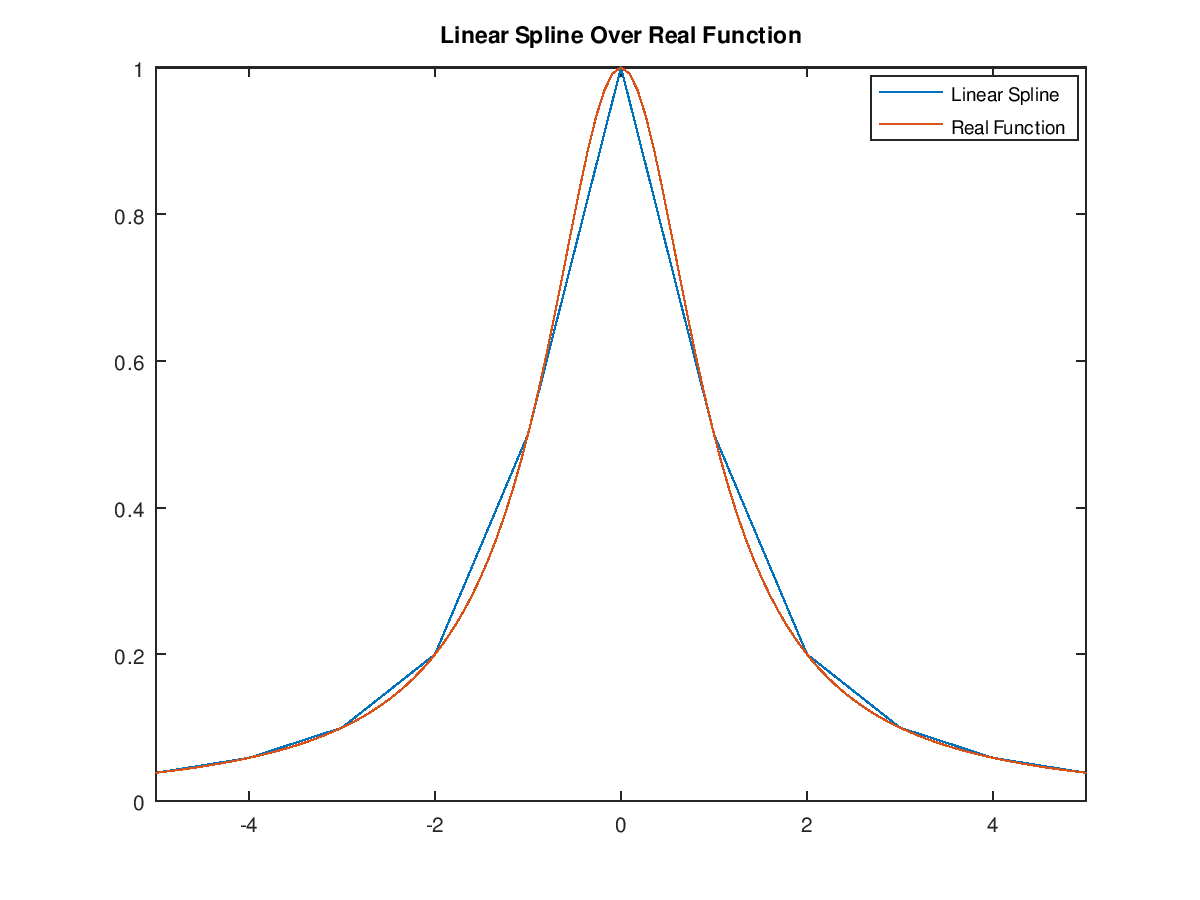
\includegraphics[width=0.8\textwidth, height=0.6\textwidth]{LinearSplinePlot.png}
\end{figure}

	\subsection{Natural Cubic spline function:}
	\subsection{Numerical approximation of the first derivative}
{\bf Area of application:}In numerical analysis, Richardson extrapolation is a sequence acceleration method, used to improve the rate of convergence of a sequence. 

{\bf Idea of the method:} 
Suppose that we wish to approximate$A^* A^* $, and we have a method $
 {\displaystyle A(h)} $that depends on a small parameter $ h $ in such a way that\\
$A ( h ) = A ^ { * } + C h ^ { n } + O \left( h ^ { n + 1 } \right)$\\
\\
From this we can get the function:\\
$R ( h , t ) = \frac { t ^ { n } \left( A ^ { * } + C \left( \frac { h } { t } \right) ^ { n } + O \left( h ^ { n + 1 } \right) \right) - \left( A ^ { * } + C h ^ { n } + O \left( h ^ { n + 1 } \right) \right) } { t ^ { n } - 1 } = A ^ { * } + O \left( h ^ { n + 1 } \right)$
{\\\bf Code:}
\begin{verbatim}
tStart = 0          %Starting time
tEnd = 5            %Ending time
f = -y^2            %The derivative of y, so y' = f(t, y(t)) = -y^2
% The solution to this ODE is y = 1/(1 + t)
y0 = 1              %The initial position (i.e. y0 = y(tStart) = y(0) = 1)
tolerance = 10^-11  %10 digit accuracy is desired

maxRows = 20                %Don't allow the iteration to continue indefinitely
initialH = tStart - tEnd    %Pick an initial step size
haveWeFoundSolution = false %Were we able to find the solution to within the desired tolerance? not yet.

h = initialH

%Create a 2D matrix of size maxRows by maxRows to hold the Richardson extrapolates
%Note that this will be a lower triangular matrix and that at most two rows are actually
% needed at any time in the computation.
A = zeroMatrix(maxRows, maxRows)

%Compute the top left element of the matrix
A(1, 1) = Trapezoidal(f, tStart, tEnd, h, y0)

%Each row of the matrix requires one call to Trapezoidal
%This loops starts by filling the second row of the matrix, since the first row was computed above
for i = 1 : maxRows - 1 %Starting at i = 1, iterate at most maxRows - 1 times
h = h/2             %Half the previous value of h since this is the start of a new row

%Call the Trapezoidal function with this new smaller step size
A(i + 1, 1) = Trapezoidal(f, tStart, tEnd, h, y0)

for j = 1 : i         %Go across the row until the diagonal is reached
%Use the value just computed (i.e. A(i + 1, j)) and the element from the
% row above it (i.e. A(i, j)) to compute the next Richardson extrapolate

A(i + 1, j + 1) = ((4^j).*A(i + 1, j) - A(i, j))/(4^j - 1);
end

%After leaving the above inner loop, the diagonal element of row i + 1 has been computed
% This diagonal element is the latest Richardson extrapolate to be computed  
%The difference between this extrapolate and the last extrapolate of row i is a good
% indication of the error
if(absoluteValue(A(i + 1, i + 1) - A(i, i)) < tolerance)   %If the result is within tolerance
print("y(5) = ", A(i + 1, i + 1))                      %Display the result of the Richardson extrapolation
haveWeFoundSolution = true
break                                                  %Done, so leave the loop
end
end

if(haveWeFoundSolution == false)   %If we weren't able to find a solution to within the desired tolerance
print("Warning: Not able to find solution to within the desired tolerance of ", tolerance);
print("The last computed extrapolate was ", A(maxRows, maxRows))
end
\end{verbatim}
{\bf Numerical analysis}
\begin{itemize}
	\item{\bf When does it converge:} Provided we have the proper data; always converges.
	\item {\bf Error estimate:}
	\begin{equation}
	\begin{split}
	&K h ^ { 2 } + O \left( h ^ { 3 } \right)
	\end{split}
	\end{equation}
	\item {\bf Pros \& Cons:}
	\begin{itemize}
		\item Intuitive
		\item Accurate
		\item Powerful Tool
	\end{itemize}
\end{itemize}
{\bf Numerical experiment:}
$f ^ { \prime } ( x ) \approx \frac { 1 } { 4 h } ( f ( x + 2 h ) - f ( x - 2 h ) )$\\
We then get the following:\\
 $f(x+2h) = f(x) + 2hf'(x) + \frac{4h^2}{2!}f''(x) + \frac{8h^3}{3!}f'''(x)\newline
f(x-2h) = f(x) - 2hf'(x) + \frac{4h^2}{2!}f''(x) - \frac{8h^3}{3!}f'''(x)\newline
f(x+2h) - f(x-2h) = 4hf'(x) + \frac{8h^3}{3!}f'''(\zeta) + \frac{8h^3}{3!}f'''(\xi)\newline
f'(x) - \frac{f(x+2h) - f(x-2h)}{4h} = \frac{8h^2}{4!}f'''(\zeta) + \frac{8h^2}{4!}f'''(\xi)\\$
$\\f(x+2h) = f(x) + 2hf'(x) + \frac{4h^2}{2!}f''(x) + \frac{8h^3}{3!}f'''(x) + \frac{16h^4}{4!}f''''(x)\\
f(x-2h) = f(x) - 2hf'(x) + \frac{4h^2}{2!}f''(x) - \frac{8h^3}{3!}f'''(x) + \frac{16h^4}{4!}f''''(x)\\
f(x+2h)+f(x-2h)=2f(x)+\frac{8h^2}{2!}f''(x) +\frac{16h^4}{4!}f''''(\zeta) +\frac{16h^4}{4!}f''''(\xi)\\
f(x+2h)+f(x-2h)-2f(x) =\frac{8h^2}{2!}f''(x) +\frac{16h^4}{4!}f''''(\zeta) +\frac{16h^4}{4!}f''''(\xi)\\
\frac{f(x+2h)+f(x-2h)-2f(x)}{4h^2} = f''(x) +\frac{4h^2}{4!}f''''(\zeta) +\frac{4h^2}{4!}f''''(\xi)\\
\frac{f(x+2h)+f(x-2h)-2f(x)}{4h^2} - f''(x) =\frac{4h^2}{4!}f''''(\zeta) +\frac{4h^2}{4!}f''''(\xi)\\
$
$\\x-2h \leq \zeta \leq x\\x \leq \xi \leq x+2h$

The graph is
\begin{figure}[H]
	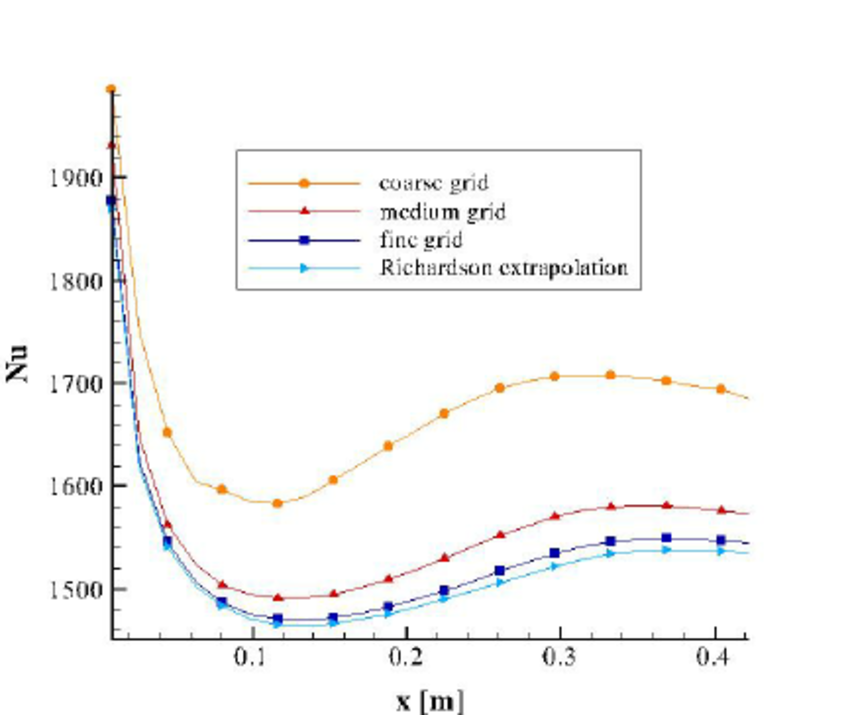
\includegraphics[width=0.8\textwidth, height=0.6\textwidth]{rich-extrap.png}
\end{figure}
	\subsection{Numerical integration using left point formula and midpoint formula}
{\bf Area of application:}Used to find a numerical approximation for a definite integral

{\bf Idea of the method:} 
Take the sum of the area under the curve by splitting the region into shapes. Take the shapes that together form a region that is similar to the region being measured, then calculating the area for each of these shapes, and finally adding all of these small areas together. 
{\\\bf Code:}
\begin{verbatim}
x1 = 1;
x2 = 3;
f=@(x)  2*x.^5 - 3*x.^2 - 5;
n=500;
dx=(x2-x1)/n;
summe=0.0;
for i=1:500
summe=summe+f(x1+dx*(i-1));
end
summe=summe*dx;
z=integral(f,x1,x2);


  dx = (b-a)/N;
sum_mdp = 0;
for p = 1:N
X = a + p*(dx)-(dx/2); 
Y = sqrt(((X^2)-(c^2)))/X;
sum_mdp = sum_mdp + Y*dx;      
end
Int_mdp(N) = sum_mdp;

\end{verbatim}
{\bf Numerical analysis}
\begin{itemize}
	\item{\bf When does it converge:} Provided we have the proper data and a continuous function with no gaps; always converges.
	\item {\bf Error estimate:}
	\begin{equation}
	\begin{split}
	&\Delta x | f ( b ) - f ( a ) |\\
	\\
	\frac{(h/2)^\xi}{3!}f'''(M)
	\end{split}
	\end{equation}
	\item {\bf Pros \& Cons:}
	\begin{itemize}
		\item Intuitive
		\item Simple to Use
		\item Requires very small shapes to remain accurate
	\end{itemize}
\end{itemize}
{\bf Numerical experiment:}
$ f(x)=x^2-x $ from $ -1$ to 3 with $ n=4 $.\\
Left:\\
$= f ( - 1 ) \cdot 1 + f ( 0 ) \cdot 1 + f ( 1 ) \cdot 1 + f ( 2 ) \cdot 1$\\
$= - 2 + 0 + 0 + 6$\\
$= 4$\\
Mid:\\
$\begin{aligned} f \left( \frac { x _ { 0 } + x _ { 1 } } { 2 } \right) & = f \left( \frac { ( - 1 ) + ( 0 ) } { 2 } \right) = f \left( - \frac { 1 } { 2 } \right) = \frac { 3 } { 4 } = 0.75 \\ f \left( \frac { x _ { 1 } + x _ { 2 } } { 2 } \right) & = f \left( \frac { ( 0 ) + ( 1 ) } { 2 } \right) = f \left( \frac { 1 } { 2 } \right) = - \frac { 1 } { 4 } = - 0.25 \\ f \left( \frac { x _ { 2 } + x _ { 3 } } { 2 } \right) & = f \left( \frac { ( 1 ) + ( 2 ) } { 2 } \right) = f \left( \frac { 3 } { 2 } \right) = \frac { 3 } { 4 } = 0.75 \\ f \left( \frac { x _ { 3 } + x _ { 4 } } { 2 } \right) & = f \left( \frac { ( 2 ) + ( 3 ) } { 2 } \right) = f \left( \frac { 5 } { 2 } \right) = \frac { 15 } { 4 } = 3.75 \end{aligned}$\\
\\
$1 ( 0.75 - 0.25 + 0.75 + 3.75 ) $ \\
$= 5$

The graph is
\begin{figure}[H]
	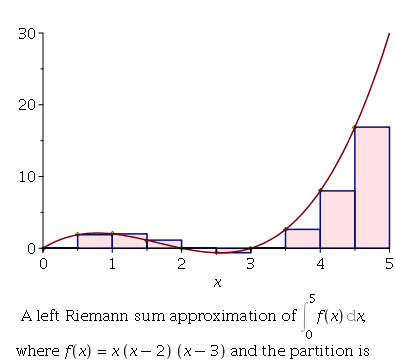
\includegraphics[width=0.8\textwidth, height=0.6\textwidth]{left_rei.png}
	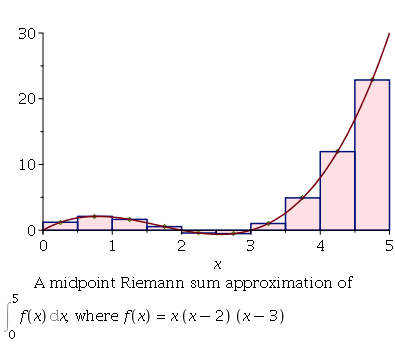
\includegraphics[width=0.8\textwidth, height=0.6\textwidth]{mid_rei.png}
\end{figure}

	\subsection{Trapezoid Rule}
{\bf Area of application:}Used to find a numerical approximation for a definite integral

{\bf Idea of the method:} 
Take the sum of the area under the curve by splitting the region into shapes. Take the shapes that together form a region that is similar to the region being measured, then calculating the area for each of these shapes, and finally adding all of these small areas together. 
{\\\bf Code:}
\begin{verbatim}
function y = Trap (f, a, b, n)
h = abs((b-a)/n);
y = 0;
for i = a:h:b
if (i==a || i==b)
y+=(h/2)*f(i);
elseif
y+=(h.*f(i));
endif
endfor
endfunction
\end{verbatim}
{\bf Numerical analysis}
\begin{itemize}
	\item{\bf When does it converge:} Provided we have the proper data and a continuous function with no gaps; always converges.
	\item {\bf Error estimate:}
	\begin{equation}
	\begin{split}
	&\Delta x | f ( b ) - f ( a ) |\\
	\\
	(h/2)f(x_i)+(h/2)f(x_{i+1})
	\end{split}
	\end{equation}
	\item {\bf Pros \& Cons:}
	\begin{itemize}
		\item Intuitive
		\item Simple to Use
		\item Requires very small shapes to remain accurate
	\end{itemize}
\end{itemize}
{\bf Numerical experiment:}
$ f(x)=x^2-x $ from $ -1$ to 3 with $ n=4 $.\\
\\
$f \left( x _ { 0 } \right) = f ( a ) = f ( - 1 ) = 2 = 2$
$2 f \left( x _ { 1 } \right) = 2 f ( 0 ) = 0 = 0$
$2 f \left( x _ { 2 } \right) = 2 f ( 1 ) = 0 = 0$
$2 f \left( x _ { 3 } \right) = 2 f ( 2 ) = 4 = 4$
$f \left( x _ { 4 } \right) = f ( b ) = f ( 3 ) = 6 = 6$\\
\\
$\frac { 1 } { 2 } ( 2 + 0 + 0 + 4 + 6 ) = 6$
The graph is
\begin{figure}[H]
	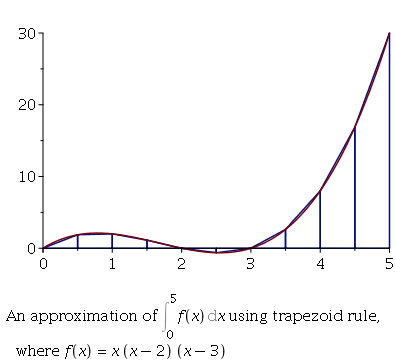
\includegraphics[width=0.8\textwidth, height=0.6\textwidth]{trap_rei.png}
\end{figure}
	\subsection{Simpson's Rule}
{\bf Area of application:}Used to find a numerical approximation for a definite integral

{\bf Idea of the method:} 
Take the sum of the area under the curve by splitting the region into shapes. Take the shapes that together form a region that is similar to the region being measured, then calculating the area for each of these shapes, and finally adding all of these small areas together. \\
$\frac { \Delta x } { 3 } \left( f \left( x _ { 0 } \right) + 4 f \left( x _ { 1 } \right) + 2 f \left( x _ { 2 } \right) + 4 f \left( x _ { 3 } \right) + 2 f \left( x _ { 4 } \right) + \cdots + 4 f \left( x _ { n - 1 } \right) + f \left( x _ { n } \right) \right)$
{\\\bf Code:}
\begin{verbatim}
function y = Simpson (f, a, b, n)
hBar = abs((b-a)/n);
h = hBar/2;
y=0;
for i = a:hBar:b-hBar
y+=(h/3)*(f(i)+4*f(i+h)+f(i+(2*h)));
endfor
endfunction
\end{verbatim}
{\bf Numerical analysis}
\begin{itemize}
	\item{\bf When does it converge:} Provided we have the proper data and a continuous function with no gaps; always converges.
	\item {\bf Error estimate:}
	\begin{equation}
	\begin{split}
&- \frac { 1 } { 90 } \left( \frac { b - a } { n } \right) ^ { 5 } f ^ { ( 4 ) } ( \xi )
	\end{split}
	\end{equation}
	\item {\bf Pros \& Cons:}
	\begin{itemize}
		\item Intuitive
		\item Simple to Use
		\item Requires very small shapes to remain accurate
	\end{itemize}
\end{itemize}
{\bf Numerical experiment:}
$ f(x)=x^2-x $ from $ -1$ to 3 with $ n=4 $.\\
\\
$f \left( x _ { 0 } \right) = f ( a ) = f ( - 1 ) = 2 = 2$
$4 f \left( x _ { 1 } \right) = 4 f ( 0 ) = 0 = 0$
$2 f \left( x _ { 2 } \right) = 2 f ( 1 ) = 0 = 0$
$4 f \left( x _ { 3 } \right) = 4 f ( 2 ) = 8 = 8$
$f \left( x _ { 4 } \right) = f ( b ) = f ( 3 ) = 6 = 6$
\\
$\frac { 1 } { 3 } ( 2 + 0 + 0 + 8 + 6 ) = 5.33333333333333$
The graph is
\begin{figure}[H]
	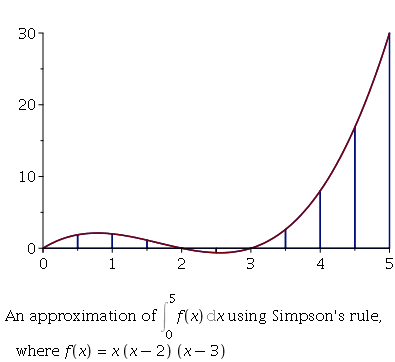
\includegraphics[width=0.8\textwidth, height=0.6\textwidth]{simp.png}
\end{figure}
	\subsection{Adaptive Simpson's rule}
{\bf Area of application:}Used to find a numerical approximation for a definite integral

{\bf Idea of the method:} 
 Adaptive Simpson's method uses an estimate of the error we get from calculating a definite integral using Simpson's rule. If the error exceeds a user-specified tolerance, the algorithm calls for subdividing the interval of integration in two and applying adaptive Simpson's method to each subinterval in a recursive manner
{\\\bf Code:}
Python.
\begin{verbatim}
from __future__ import division # python 2 compat
# "structured" adaptive version, translated from Racket
def _quad_simpsons_mem(f, a, fa, b, fb):
"""Evaluates the Simpson's Rule, also returning m and f(m) to reuse"""
m = (a+b) / 2
fm = f(m)
return (m, fm, abs(b-a) / 6 * (fa + 4 * fm + fb))

def _quad_asr(f, a, fa, b, fb, eps, whole, m, fm):
"""
Efficient recursive implementation of adaptive Simpson's rule.
Function values at the start, middle, end of the intervals are retained.
"""
lm, flm, left  = _quad_simpsons_mem(f, a, fa, m, fm)
rm, frm, right = _quad_simpsons_mem(f, m, fm, b, fb)
delta = left + right - whole
if abs(delta) <= 15 * eps:
return left + right + delta / 15
return _quad_asr(f, a, fa, m, fm, eps/2, left , lm, flm) +\
_quad_asr(f, m, fm, b, fb, eps/2, right, rm, frm)

def quad_asr(f, a, b, eps):
"""Integrate f from a to b using Adaptive Simpson's Rule with max error of eps."""
fa, fb = f(a), f(b)
m, fm, whole = _quad_simpsons_mem(f, a, fa, b, fb)
return _quad_asr(f, a, fa, b, fb, eps, whole, m, fm)

from math import sin
print(quad_asr(sin, 0, 1, 1e-09))
\end{verbatim}
{\bf Numerical analysis}
\begin{itemize}
	\item{\bf When does it converge:} Provided we have the proper data and a continuous function with no gaps; always converges.
	\item {\bf Error estimate:}
	\begin{equation}
	\begin{split}
&- \frac { 1 } { 90 } \left( \frac { b - a } { n } \right) ^ { 5 } f ^ { ( 4 ) } ( \xi )
	\end{split}
	\end{equation}
	\item {\bf Pros \& Cons:}
	\begin{itemize}
		\item Intuitive
		\item Simple to Use
		\item Fewer functions than before
	\end{itemize}
\end{itemize}
{\bf Numerical experiment:}

Consider the integral  $\int _ { 1 } ^ { 3 } e ^ { 2 x } \sin 3 x d x$\\
$\begin{aligned} S ( 1,3 ) & = 35.42697658812284 \\ S ( 1,2 ) & = - 15.45828245392933 \\ S ( 2,3 ) & = 117.9751755250024 \end{aligned}$\\
Continuing:\\
$\begin{aligned} S ( 1,2 ) & = - 15.45828245392933 \\ S ( 1,1.5 ) & = - 3.87030357255464 \\ S ( 1.5,2 ) & = - 12.38881686458909 \end{aligned}$\\
The final approx for the problem is \\
$S ( 1,1.5 ) + S ( 1.5,2 ) + S ( 2,2.25 ) + S ( 2.25,2.5 ) + S ( 2.5,2.75 ) + S ( 2.75,3 )$
Thus, 108.5722885413671
	\subsection{Gaussian Quadrature Formula}
{\bf Area of application:}Quadrature rule is an approximation of the definite integral of a function, usually stated as a weighted sum of function values at specified points within the domain of integration

{\bf Idea of the method:} 
$ Pn(x) $. With the n-th polynomial normalized to give $ Pn(1) = 1 $, the i-th Gauss node, xi, is the i-th root of Pn and the weights are given by the formula

$ {\displaystyle w_{i}={\frac {2}{\left(1-x_{i}^{2}\right)[P'_{n}(x_{i})]^{2}}}.} w_{i}={\frac {2}{\left(1-x_{i}^{2}\right)[P'_{n}(x_{i})]^{2}}}. $
{\\\bf Code:}
\begin{verbatim}
function [x,w]=lgwt(N,a,b)
% lgwt.m
%
% This script is for computing definite integrals using Legendre-Gauss 
% Quadrature. Computes the Legendre-Gauss nodes and weights  on an interval
% [a,b] with truncation order N
%
% Suppose you have a continuous function f(x) which is defined on [a,b]
% which you can evaluate at any x in [a,b]. Simply evaluate it at all of
% the values contained in the x vector to obtain a vector f. Then compute
% the definite integral using sum(f.*w);
%
% Written by Greg von Winckel - 02/25/2004
N=N-1;
N1=N+1; N2=N+2;
xu=linspace(-1,1,N1)';
% Initial guess
y=cos((2*(0:N)'+1)*pi/(2*N+2))+(0.27/N1)*sin(pi*xu*N/N2);
% Legendre-Gauss Vandermonde Matrix
L=zeros(N1,N2);
% Derivative of LGVM
Lp=zeros(N1,N2);
% Compute the zeros of the N+1 Legendre Polynomial
% using the recursion relation and the Newton-Raphson method
y0=2;
% Iterate until new points are uniformly within epsilon of old points
while max(abs(y-y0))>eps


L(:,1)=1;
Lp(:,1)=0;

L(:,2)=y;
Lp(:,2)=1;

for k=2:N1
L(:,k+1)=( (2*k-1)*y.*L(:,k)-(k-1)*L(:,k-1) )/k;
end

Lp=(N2)*( L(:,N1)-y.*L(:,N2) )./(1-y.^2);   

y0=y;
y=y0-L(:,N2)./Lp;

end
% Linear map from[-1,1] to [a,b]
x=(a*(1-y)+b*(1+y))/2;      
% Compute the weights
w=(b-a)./((1-y.^2).*Lp.^2)*(N2/N1)^2;
\end{verbatim}
{\bf Numerical analysis}
\begin{itemize}
	\item{\bf When does it converge:} Provided we have the proper data; always converges.
	\item {\bf Error estimate:}
	\begin{equation}
	\begin{split}
	&\frac { f ^ { ( 2 n ) } ( \xi ) } { ( 2 n ) ! } \left( p _ { n } , p _ { n } \right)
	\end{split}
	\end{equation}
	\item {\bf Pros \& Cons:}
	\begin{itemize}
		\item Intuitive
		\item Super Accurate
		\item Fast
	\end{itemize}
\end{itemize}
{\bf Numerical experiment:}
Gaussian Quadrature of $ \sin(x), 0, \pi $\\$\begin{array} { l } { \text { Gaussian Quadrature } } \\ { 0.064180425349 } \\ { 0.001388913608 } \\ { 0.000015771542 } \\ { 0.000000110284 } \\ { 0.000000000523 } \end{array}$\\
The graph is
\begin{figure}[H]
	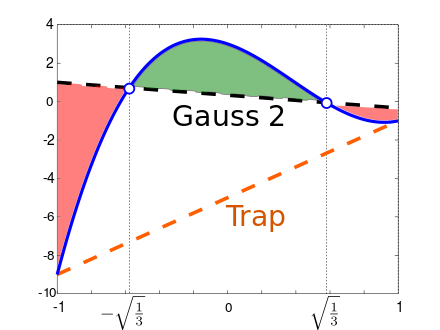
\includegraphics[width=0.8\textwidth, height=0.6\textwidth]{g_quad.png}
\end{figure}
{\bf Area of application:}Quadrature rule is an approximation of the definite integral of a function, usually stated as a weighted sum of function values at specified points within the domain of integration

{\bf Idea of the method:} 
$ Pn(x) $. With the n-th polynomial normalized to give $ Pn(1) = 1 $, the i-th Gauss node, xi, is the i-th root of Pn and the weights are given by the formula

$ {\displaystyle w_{i}={\frac {2}{\left(1-x_{i}^{2}\right)[P'_{n}(x_{i})]^{2}}}.} w_{i}={\frac {2}{\left(1-x_{i}^{2}\right)[P'_{n}(x_{i})]^{2}}}. $
{\\\bf Code:}
\begin{verbatim}
function [x,w]=lgwt(N,a,b)
% lgwt.m
%
% This script is for computing definite integrals using Legendre-Gauss 
% Quadrature. Computes the Legendre-Gauss nodes and weights  on an interval
% [a,b] with truncation order N
%
% Suppose you have a continuous function f(x) which is defined on [a,b]
% which you can evaluate at any x in [a,b]. Simply evaluate it at all of
% the values contained in the x vector to obtain a vector f. Then compute
% the definite integral using sum(f.*w);
%
% Written by Greg von Winckel - 02/25/2004
N=N-1;
N1=N+1; N2=N+2;
xu=linspace(-1,1,N1)';
% Initial guess
y=cos((2*(0:N)'+1)*pi/(2*N+2))+(0.27/N1)*sin(pi*xu*N/N2);
% Legendre-Gauss Vandermonde Matrix
L=zeros(N1,N2);
% Derivative of LGVM
Lp=zeros(N1,N2);
% Compute the zeros of the N+1 Legendre Polynomial
% using the recursion relation and the Newton-Raphson method
y0=2;
% Iterate until new points are uniformly within epsilon of old points
while max(abs(y-y0))>eps


L(:,1)=1;
Lp(:,1)=0;

L(:,2)=y;
Lp(:,2)=1;

for k=2:N1
L(:,k+1)=( (2*k-1)*y.*L(:,k)-(k-1)*L(:,k-1) )/k;
end

Lp=(N2)*( L(:,N1)-y.*L(:,N2) )./(1-y.^2);   

y0=y;
y=y0-L(:,N2)./Lp;

end
% Linear map from[-1,1] to [a,b]
x=(a*(1-y)+b*(1+y))/2;      
% Compute the weights
w=(b-a)./((1-y.^2).*Lp.^2)*(N2/N1)^2;
\end{verbatim}
{\bf Numerical analysis}
\begin{itemize}
	\item{\bf When does it converge:} Provided we have the proper data; always converges.
	\item {\bf Error estimate:}
	\begin{equation}
	\begin{split}
	&\frac { f ^ { ( 2 n ) } ( \xi ) } { ( 2 n ) ! } \left( p _ { n } , p _ { n } \right)
	\end{split}
	\end{equation}
	\item {\bf Pros \& Cons:}
	\begin{itemize}
		\item Intuitive
		\item Super Accurate
		\item Fast
	\end{itemize}
\end{itemize}
{\bf Numerical experiment:}
Gaussian Quadrature of $ \sin(x), 0, \pi $\\$\begin{array} { l } { \text { Gaussian Quadrature } } \\ { 0.064180425349 } \\ { 0.001388913608 } \\ { 0.000015771542 } \\ { 0.000000110284 } \\ { 0.000000000523 } \end{array}$\\
The graph is
\begin{figure}[H]
	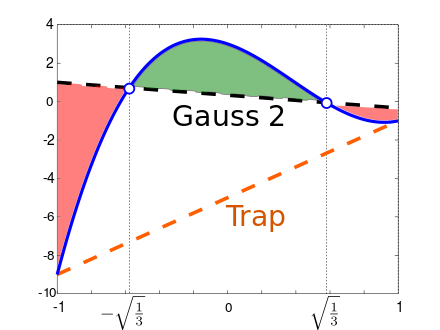
\includegraphics[width=0.8\textwidth, height=0.6\textwidth]{g_quad.png}
\end{figure}
	\subsection{Naive Gaussian Elimination}
{\bf Area of application:}An algorithm for solving systems of linear equations. It is usually understood as a sequence of operations performed on the corresponding matrix of coefficients. This method can also be used to find the rank of a matrix, to calculate the determinant of a matrix, and to calculate the inverse of an invertible square matrix. 

{\bf Idea of the method:} 
To perform row reduction on a matrix, one uses a sequence of elementary row operations to modify the matrix until the lower left-hand corner of the matrix is filled with zeros, as much as possible.
{\\\bf Code:}
\begin{verbatim}
function Aug = GaussianElimination (A, b)
ACol = columns(A);
ARows = rows(A);
Aug = [A b];
AugCol = columns(Aug);
for i = 1:ACol
pivotVal = Aug(i,i);
for j = i+1:ARows
underVal = Aug(j, i);
for k = i:AugCol
Aug(j, k) = Aug(j, k) - (underVal/pivotVal)*Aug(i, k);
endfor
endfor
endfor
endfunction
\end{verbatim}
{\bf Numerical analysis}
\begin{itemize}
	\item{\bf When does it converge:} Provided we have the proper data; always converges.
	\item {\bf Error estimate:}
	\begin{equation}
	\begin{split}
	&\frac { f ^ { ( 2 n ) } ( \xi ) } { ( 2 n ) ! } \left( p _ { n } , p _ { n } \right)
	\end{split}
	\end{equation}
	\item {\bf Pros \& Cons:}
	\begin{itemize}
		\item Intuitive
		\item Slow
		\item Easy to implement
	\end{itemize}
\end{itemize}
{\bf Numerical experiment:}
$\left[
\begin{array}{cccc|c}
6 & -2 & 2 & 4 & 16 \\
12 & -8 & 6 & 10 & 26 \\
3 & -13 & 9 & 3 & -19 \\
-6 & 4 & 1 & -18 & -34\\
\end{array}
\right]
\rightarrow
\left[
\begin{array}{cccc|c}
6 & -2 & 2 & 4 & 16 \\
0 & -4 & 2 & 2 & -6 \\
0 & -12 & 8 & 1 & -27 \\
0 & 2 & 1 & -14 & -18\\
\end{array}
\right]
\rightarrow
\left[
\begin{array}{cccc|c}
6 & -2 & 2 & 4 & 16 \\
0 & -4 & 2 & 2 & -6 \\
0 & 0 & 2 & -5 & -9 \\
0 & 0 & 4 & -13 & -21\\
\end{array}
\right]
\rightarrow
\left[
\begin{array}{cccc|c}
6 & -2 & 2 & 4 & 16 \\
0 & -4 & 2 & 2 & -6 \\
0 & 0 & 2 & -5 & -9 \\
0 & 0 & 0 & -3 & -3\\
\end{array}
\right]
$

$\vec{x} = \begin{bmatrix} 
3\\
1 \\
-2\\
1
\end{bmatrix}\\
$
	\subsection{Gaussian Elimination partial and full pivoting}
{\bf Area of application:}An algorithm for solving systems of linear equations. It is usually understood as a sequence of operations performed on the corresponding matrix of coefficients. This method can also be used to find the rank of a matrix, to calculate the determinant of a matrix, and to calculate the inverse of an invertible square matrix. 

{\bf Idea of the method:} 
To perform row reduction on a matrix, one uses a sequence of elementary row operations to modify the matrix until the lower left-hand corner of the matrix is filled with zeros, as much as possible.
{\\\bf Code:}
\begin{verbatim}
function [Aug swaps]= GaussianEliminationPartial (A, b)
ACol = columns(A);
ARows = rows(A);
Aug = [A b];
AugCol = columns(Aug);
swaps = zeros(0, 2);
for i = 1:ACol
maxIdx = MaxColValIdx(Aug(:, i), i);
swaps = [swaps ; i maxIdx];
tmpCurrPivot = Aug(i, :);
Aug
Aug(i, :) = Aug(maxIdx, :);
Aug(maxIdx, :) = tmpCurrPivot;
Aug
pivotVal = Aug(i,i)
for j = i+1:ARows
underVal = Aug(j, i);
for k = i:AugCol
Aug(j, k) = Aug(j, k) - (underVal/pivotVal)*Aug(i, k);
endfor
endfor
endfor
swaps
endfunction

function idx = MaxColValIdx (currCol, start)
idx = start;
maxVal = abs(currCol(idx));
for i = start:length(currCol)
if(abs(currCol(i))>maxVal)
maxVal = abs(currCol(i));
idx = i;
endif
endfor
endfunction
\end{verbatim}
{\bf Numerical analysis}
\begin{itemize}
	\item{\bf When does it converge:} Provided we have the proper data; always converges.
	\item {\bf Error estimate:}
	\begin{equation}
	\begin{split}
	& e_n+f(\xi)
	\end{split}
	\end{equation}
	\item {\bf Pros \& Cons:}
	\begin{itemize}
		\item Intuitive
		\item Faster than naive elimination
	\end{itemize}
\end{itemize}
{\bf Numerical experiment:}
$\left[
\begin{array}{cccc|c}
6 & -2 & 2 & 4 & 16 \\
12 & -8 & 6 & 10 & 26 \\
3 & -13 & 9 & 3 & -19 \\
-6 & 4 & 1 & -18 & -34\\
\end{array}
\right]
\rightarrow
\left[
\begin{array}{cccc|c}
6 & -2 & 2 & 4 & 16 \\
0 & -4 & 2 & 2 & -6 \\
0 & -12 & 8 & 1 & -27 \\
0 & 2 & 1 & -14 & -18\\
\end{array}
\right]
\rightarrow
\left[
\begin{array}{cccc|c}
6 & -2 & 2 & 4 & 16 \\
0 & -4 & 2 & 2 & -6 \\
0 & 0 & 2 & -5 & -9 \\
0 & 0 & 4 & -13 & -21\\
\end{array}
\right]
\rightarrow
\left[
\begin{array}{cccc|c}
6 & -2 & 2 & 4 & 16 \\
0 & -4 & 2 & 2 & -6 \\
0 & 0 & 2 & -5 & -9 \\
0 & 0 & 0 & -3 & -3\\
\end{array}
\right]
$

$\vec{x} = \begin{bmatrix} 
3\\
1 \\
-2\\
1
\end{bmatrix}\\
$
	\subsection{LU factorization}
{\bf Area of application:}Factors a matrix as the product of a lower triangular matrix and an upper triangular matrix. The product sometimes includes a permutation matrix as well. LU decomposition can be viewed as the matrix form of Gaussian elimination. 

{\bf Idea of the method:} 
Let $ A = LU $ where $ L $ is a lower triangular matrix and $ U $ is an upper triangular matrix. Use Gaussian elimination as normal.
{\\\bf Code:}
\begin{verbatim}
function [L U] = LUDecomposition (A)
ACol = columns(A);
ARows = rows(A);
U = A;
L = eye(columns(A));
UCol = columns(U);
for i = 1:ACol
pivotVal = U(i,i);
for j = i+1:ARows
underVal = U(j, i);
for k = i:UCol
U(j, k) = U(j, k) - (underVal/pivotVal)*U(i, k);
L(j, k) = L(j, k) + (underVal/pivotVal)*L(i, k);
endfor
endfor
endfor
endfunction
\end{verbatim}
{\bf Numerical analysis}
\begin{itemize}
	\item{\bf When does it converge:} Provided we have the proper data; always converges.
	\item {\bf Error estimate:}
	\begin{equation}
	\begin{split}
	& e_n+f(\xi)
	\end{split}
	\end{equation}
	\item {\bf Pros \& Cons:}
	\begin{itemize}
		\item Intuitive
		\item Nice Structure
		\item Hard to setup
	\end{itemize}
\end{itemize}
{\bf Numerical experiment:}
   We start by reducing A to echelon form to produce U.\\
\[A = \begin{bmatrix} 
6 & -2 & 2 & 4\\
12 & -8 & 6 & 10\\
3 & -13 & 9 & 3\\
-6 & 4 & 1 & -18
\end{bmatrix} \rightarrow \begin{bmatrix} 
6 & -2 & 2 & 4\\
0 & -4 & 2 & 2\\
0 & -12 & 8 & 1\\
0 & 2 & 3 & -14
\end{bmatrix} \rightarrow \begin{bmatrix} 
6 & -2 & 2 & 4\\
0 & -4 & 2 & 2\\
0 & 0 & 2 & -5\\
0 & 0 & 4 & -13
\end{bmatrix} \rightarrow \begin{bmatrix} 
6 & -2 & 2 & 4\\
0 & -4 & 2 & 2\\
0 & 0 & 2 & -5\\
0 & 0 & 0 & -3
\end{bmatrix} = U\]
Now we will do the inverse of the row reduction operations to the identity matrix $I$.\newline
$I = \begin{bmatrix} 
1 & 0 & 0 & 0\\
0 & 1 & 0 & 0\\
0 & 0 & 1 & 0\\
0 & 0 & 0 & 1
\end{bmatrix} \rightarrow \begin{bmatrix} 
1 & 0 & 0 & 0\\
0 & 1 & 0 & 0\\
0 & 0 & 1 & 0\\
0 & 0 & 2 & 1
\end{bmatrix} \rightarrow \begin{bmatrix} 
1 & 0 & 0 & 0\\
0 & 1 & 0 & 0\\
0 & 3 & 1 & 0\\
0 & .5 & 2 & 1
\end{bmatrix} \rightarrow \begin{bmatrix} 
1 & 0 & 0 & 0\\
2 & 1 & 0 & 0\\
.5 & 3 & 1 & 0\\
-1 & -.5 & 2 & 1
\end{bmatrix}$\newline
Now we need to solve these two equations using forward and backward substitution.\newline
$L\vec{z} = \vec{b}\\$
$U\vec{x} = \vec{z}\\$
$\\z_1 = 16\\
z_2 = 26 - 2(16) = -6\\
z_3 = -19 -0.5(16) - 3(-6) = -9\\
z_4 = -34 + 16 -0.5(-6) - 2(-9) = -3 \\$
$\vec{z} = 
\begin{bmatrix} 
16\\
-6\\
-9\\
-3\end{bmatrix}\\$
$\\U\vec{x} = \vec{z\\}$
$x_4 = -3/-3 = 1\\
x_3 = (-9 + 5(1))/2 = -2\\
x_2 = (-6 -2(1) - 2(-2))/-4 = 1\\
x_1 = (16 - 4(1)-2(-2)+2(1))/6 = 3\\
$
$\vec{x} = 
\begin{bmatrix} 
3\\
1\\
-2\\
1\end{bmatrix}\\$

	\subsection{ Forward and backward Euler's}
{\bf Area of application:}a numerical method to solve first order first degree differential equation with a given initial value 

{\bf Idea of the method:} 
The Forward Euler scheme is as follows. For $ 1 \leq n \leq N $
$ y(0) = y0 $,\\
$ \frac{dy}{dt} = F(t, y), \\ $
$ \frac{y_{n+1} − y_n}
{\Delta t} = F(t_n, y_n).\\ $
The backward Euler method computes the approximations using\\
$ {\displaystyle y_{k+1}=y_{k}+hf(t_{k+1},y_{k+1}).} y_{{k+1}}=y_{k}+hf(t_{{k+1}},y_{{k+1}}) $
{\\\bf Code:}
\begin{verbatim}
y0 = 1;
t0 = 0;
h = 1; % try: h = 0.01
tn = 4; % equal to: t0 + h*n, with n the number of steps
[t, y] = Euler(t0, y0, h, tn);
plot(t, y, 'b');

% exact solution (y = e^t):
tt = (t0:0.001:tn)';
yy = exp(tt);
hold('on');
plot(tt, yy, 'r');
hold('off');
legend('Euler', 'Exact');

function [t, y] = Euler(t0, y0, h, tn)
fprintf('%10s%10s%10s%15s\n', 'i', 'yi', 'ti', 'f(yi,ti)');
fprintf('%10d%+10.2f%+10.2f%+15.2f\n', 0, y0, t0, f(y0,t0));
t = (t0:h:tn)';
y = zeros(size(t));
y(1) = y0;
for i = 1:1:length(t)-1
y(i+1) = y(i) + h*f(y(i),t(i));
fprintf('%10d%+10.2f%+10.2f%+15.2f\n', i, y(i+1), t(i+1), f(y(i+1),t(i+1)));
end
end

% in this case, f(y,t) = f(y)
function dydt = f(y,t)
dydt = y;
end
\end{verbatim}
{\bf Numerical analysis}
\begin{itemize}
\item{\bf When does it converge:} Provided we have the proper data; always converges.
\item {\bf Error estimate:}
\begin{equation}
\begin{split}
& e_n+f(\xi)
\end{split}
\end{equation}
\item {\bf Pros \& Cons:}
\begin{itemize}
\item Intuitive
\item Backwards avoids the problems forward has
\end{itemize}
\end{itemize}
{\bf Numerical experiment:}
Here $ F(t, y) = y + 2te^{2t} $ and $ y_0 = 1. $ Since the time step is$  \Delta t = .1 $,
we need to iterate the solution twice. That is, we need to find $ y_2. $ The first iterate
gives\\
$\begin{aligned} y _ { 1 } & = y _ { 0 } + \Delta t F \left( t _ { 0 } , y _ { 0 } \right) \\ & = 1 + 0.1 \left( 1 + 2 \cdot 0 \cdot e ^ { 2 - 0 } \right) \\ & = 1.1 \end{aligned}$
and\\
$\begin{aligned} y _ { 2 } & = y _ { 1 } + \Delta t F \left( t _ { 1 } , y _ { 1 } \right) \\ & = 1.1 + 0.1 \left( 1.1 + 2 \cdot 0.1 \cdot e ^ { 2 \cdot 0.1 } \right) \\ & \simeq 1.2344 \end{aligned}$

\end{document}